\tableofcontents

\section*{Предисловие}
\indent
При выполнении данной лабораторной работы было решено использовать 
\href{https://python-control.readthedocs.io/en/0.9.4/}{Python Control Systems Library}.
Данный инструмент является альтернативой Matlab, адаптированной для использования на 
языке Python и предоставляет широкий функционал для анализа и моделирования систем,
а также синтеза регуляторов для управления.

Данная библиотека поддерживает разные формы задания систем (в том числе В-В и В-С-В).
Форма Вход-Выход задается передаточными функциями с помощью объекта 
\textbf{control.matlab.tf} (transfer function), задав числитель и знаменатель. Форма Вход-Состояние-Выход - с помощью 
\textbf{control.matlab.ss} (state space) на основе матриц. Пример задания систем приведен в коде ниже:

\begin{lstlisting}[language=Python]
import control as ctrl
import control.matlab as ctrlmat

transfer_function = ctrlmat.tf([9, 1, 2], [1, 6, 5, 2])

A = [[-6, -5, -2],
     [1, 0, 0],
     [0, 1, 0]]
B = [[1],
     [0],
     [0]]
C = [[9, 1, 2]]
D = [[0]]
state_space = ctrlmat.ss(A, B, C, D)
\end{lstlisting}

Для моделирования поведения системы в данной лабораторной использовался метод \\ 
\textbf{control.forced\_responce(sys, T=None, U=0.0, X0=0.0)}, принимающий в качестве 
аргументов систему (заданную в любой форме), дискретизированный промежуток времени, управляющее воздействие и начальные условия.
Пример моделирования:

\begin{lstlisting}[language=Python]
import numpy as np
dt = 0.001 # discretization step
modeling_time = 25 # sec
time = np.linspace(0,modeling_time_1,int(modeling_time/dt))
u = np.ones_like(time)
init_state = 0
y = ctrl.forced_response(transfer_function, U=u, X0=init_state, T=time).outputs
\end{lstlisting}
\pagebreak

\section{Одноканальная система в форме вход-выход}
В соответствии с вариантом выберем коэффициенты $a_0=2$, $a_1=5$, $a_2=6$, $b_0=2$, $b_1=1$, $b_2=9$.
Рассмотрим уравнение системы в форме В-В:
\begin{equation}
    \dddot{y} + a_2 \ddot{y} + a_1 \dot{y} + a_0 y = b_2 \ddot{u} + b_1 \dot{u} + b_0 u
\end{equation}
Можем переписать выражение в терминах дифференциальных и интегральных операторов:
\begin{equation*}
    p^3(y) + 6 p^2(y) + 5 p(y) + 2 y = 9 p^2(u) + p(u) + 2 u
\end{equation*}
Представим систему, используя передаточную функцию:
\begin{equation*}
    y(t) = \frac{9p^2 + p + 2}{p^3 + 6p^2 + 5p + 2}[u](t)
\end{equation*}

Запустим моделирование системы в python:

\begin{lstlisting}[language=Python]
transferFunction_1 = ctrlmat.tf([9, 1, 2], [1, 6, 5, 2])
modeling_time_1 = 25
time_1 = np.linspace(0,modeling_time_1,int(modeling_time_1/dt))
u_1 = np.ones_like(time_1)
init_state_1 = 0
y_1 = ctrl.forced_response(transferFunction_1, U=u_1, X0=init_state_1, T=time_1).outputs
\end{lstlisting}

\begin{figure}[h]
    \centering
    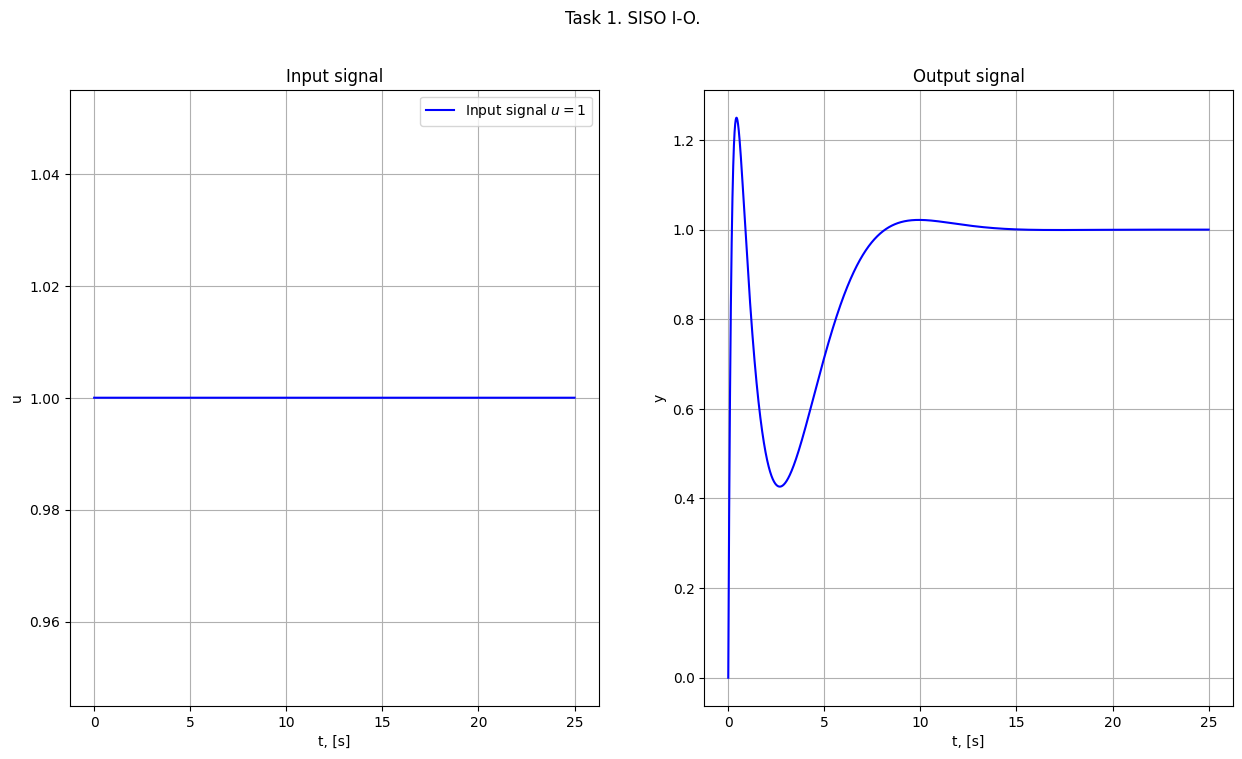
\includegraphics[width=\textwidth]{plot_1_1}
    \caption{\label{fig:The-caption-1}Входной и выходной сигналы системы (задание 1)}
\end{figure}

\pagebreak

\section{Переход от формы вход-выход к форме вход-состояние-выход}
На основе уравнения (1) зададим систему в канонической управляемой форме (reachable canonical form). В общем случае,
 систему вида $y^{(n)} + a_{n-1}y^{(n-1)} + \dots +a_0y = u^{(m)} + b_{m-1}u^{(m-1)} + \dots +b_0u, m <= n$ можем 
представить как:
\begin{equation}
    \begin{cases}
        \dot x = Ax + Bu \\
        y = Cx + Du
    \end{cases}
    A = \begin{bmatrix}
        0 & \ddots &  &  \\
        0 &  & I &  \\
        \vdots &  &  & \ddots \\
        -a_0 & -a_1 & \hdots & -a_{n-1} 
        \end{bmatrix}
        B = \begin{bmatrix}
            0 \\
            0 \\
            \vdots \\
            1
            \end{bmatrix}
        C = \begin{bmatrix}
            b_0 & b_1 & \hdots & b_{m-1}
            \end{bmatrix}
        D = \begin{bmatrix}
            \begin{cases}
                b_m, m = n \\
                0, m < n
            \end{cases}
            \end{bmatrix}
\end{equation}
Таким образом, получаем следующие матрицы, задающие систему:
\begin{equation*}
    A = \begin{bmatrix}
        0 & 1 &  0   \\
        0 &  0 & 1  \\
        -2 & -5 &  -6 
        \end{bmatrix}
        B = \begin{bmatrix}
            0  \\
            0 \\
            1
            \end{bmatrix}
        C = \begin{bmatrix}
            2 & 1 & 9
            \end{bmatrix}
        D = \begin{bmatrix}
             0
            \end{bmatrix}
\end{equation*}

Преобразуем систему в каноническую форму и выполним моделирование:
\begin{lstlisting}[language=Python]
state_space_2, _ = ctrl.canonical_form(ctrl.tf2ss(transferFunction_1),form="reachable")
u_2 = u_1.copy()
time_2 = time_1.copy()
init_state_2 = init_state_1
y_2 = ctrl.forced_response(state_space_2, U=u_1, X0=init_state_2, T=time_2).outputs
\end{lstlisting}

\begin{figure}[h]
    \centering
    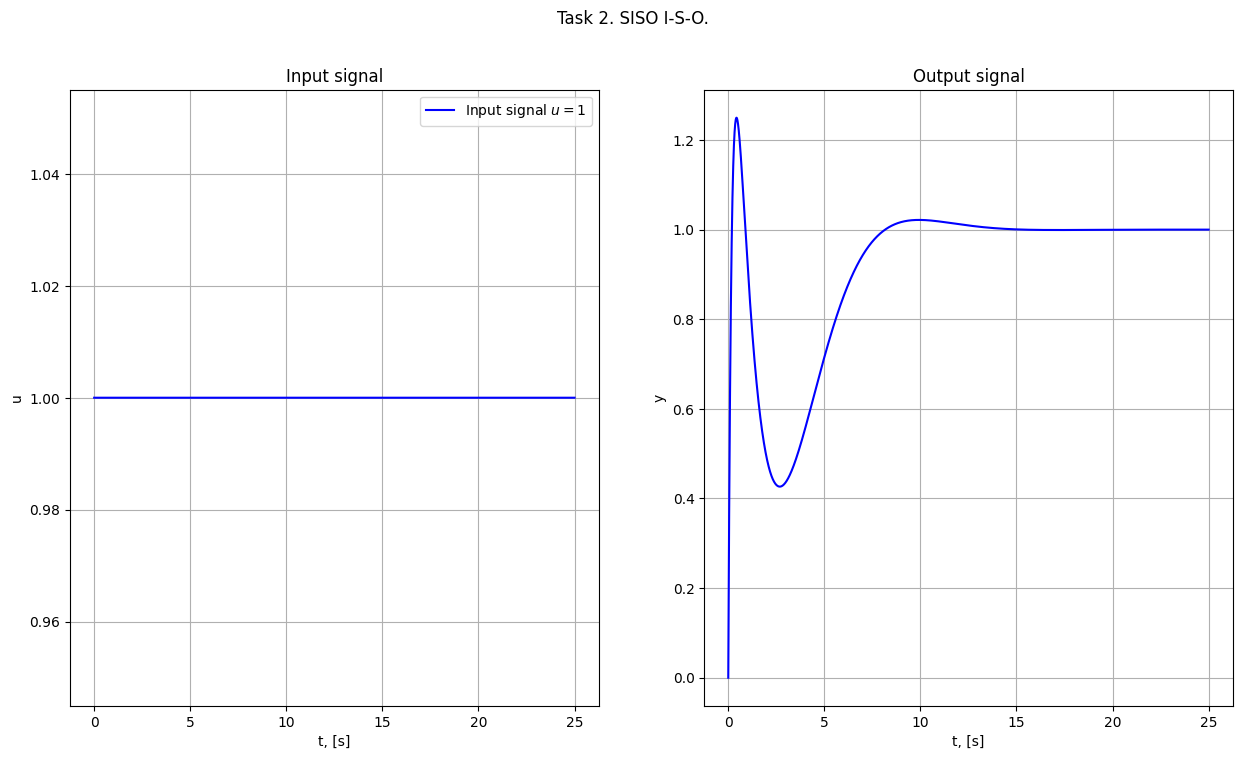
\includegraphics[width=\textwidth]{plot_2_1}
    \caption{\label{fig:The-caption-1}Входной и выходной сигналы системы (задание 2)}
\end{figure}
\begin{figure}[h]
    \centering
    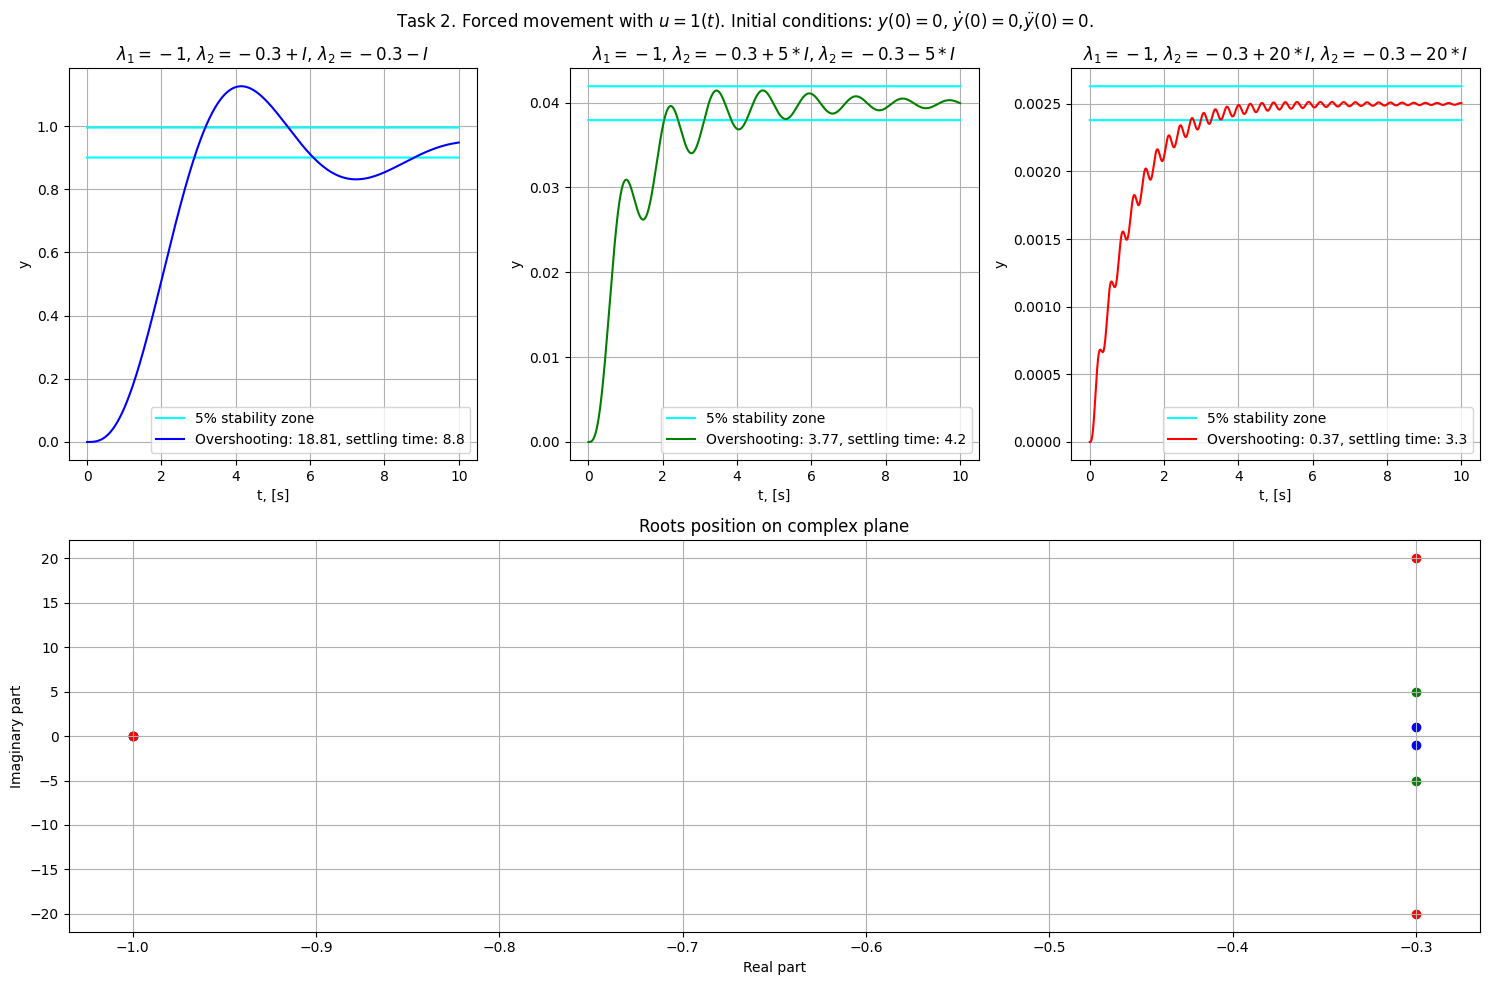
\includegraphics[width=\textwidth]{plot_2_2}
    \caption{\label{fig:The-caption-1}Сравнение выходных сигналов из заданий 1 и 2}
\end{figure}

Можем заметить, что полученный выходной сигнал совпадает с выходным сигналом 1 задания,
 что объясняется эквивалентностью систем (несмотря на разные формы их задания).

\pagebreak

\section{Многоканальная система в форме вход-выход}
Рассмотрим систему вида:
\begin{equation}
    A(p)y(t)=B(p)u(t)
\end{equation}
Приведем ее к стандартной форме В-В с помощью передаточной функции:
\begin{equation}
    y(t)=A^{-1}(p)B(p)u(t) = W[u](t)
\end{equation}

Согласно условию матрицы $A$ и $B$ имеют следующий вид:
\begin{equation*}
    A(p)= \begin{bmatrix}
        p+19 & p+3    \\
        p+6 &  p+2
        \end{bmatrix} 
    B(p)= \begin{bmatrix}
        7 & 7    \\
        5 &  6
    \end{bmatrix} 
\end{equation*}
Тогда, можем найти передаточную функцию $W(p)$:
\begin{equation*}
    W(p) = A^{-1}(p)B(p)= \frac{1}{12p + 20} \begin{bmatrix}
        p+2 & -p - 3 \\
        -p -6 & p+19
    \end{bmatrix}
    \begin{bmatrix}
        7 & 7    \\
        5 &  6
    \end{bmatrix} = \frac{1}{12p + 20} \begin{bmatrix}
        2p-1 & p - 4 \\
        -2p + 53 & -p+72
    \end{bmatrix}
\end{equation*}

Выполним моделирование системы:
\begin{lstlisting}[language=Python]
transferFunction_3 = ctrl.tf(numerators_mat, denumerators_mat)
modeling_time_3 = 20 
time_3 = np.linspace(0,modeling_time_3,int(modeling_time_3/dt))
u_3_1 = np.zeros_like(time_3) + 1
u_3_2 = 2 * np.sin(time_3)
u_3 = np.array([u_3_1, u_3_2])
init_state_3 = 0
y_3 = ctrl.forced_response(transferFunction_3, U=u_3, X0=init_state_3, T=time_3).outputs
\end{lstlisting}

\begin{figure}[h]
    \centering
    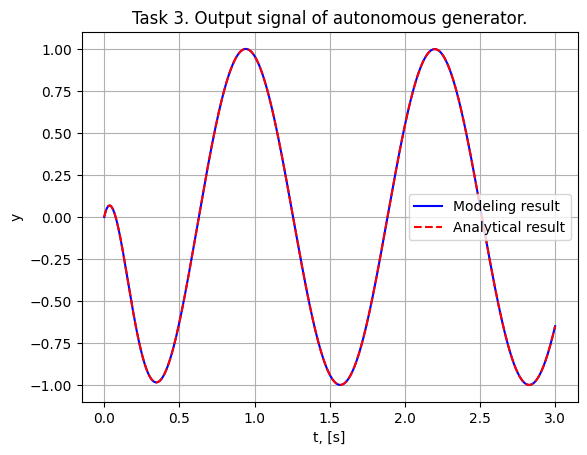
\includegraphics[width=\textwidth, height=250px]{plot_3_1}
    \caption{\label{fig:The-caption-1}Входные и выходные сигналы системы (задание 3)}
\end{figure}
\pagebreak

\section{Одноканальная система в форме вход-состояние-выход}
Рассмотрим систему вида:
\begin{equation}
    \begin{cases}
        \dot x = Ax + Bu \\
        y = Cx + Du
    \end{cases}
\end{equation}

Согласно заданию, матрицы определяющие систему имеют вид:
\begin{equation*}
    A = \begin{bmatrix}
        0 & -6   \\
        1 &  -4 
        \end{bmatrix}
        B = \begin{bmatrix}
            1  \\
            3
            \end{bmatrix}
        C = \begin{bmatrix}
            2 & 7 
            \end{bmatrix}
        D = \begin{bmatrix}
             0
            \end{bmatrix}
\end{equation*}

Выполним моделирование системы:
\begin{lstlisting}[language=Python]
state_space_4 = ctrlmat.ss(A_4, B_4, C_4, D_4)
modeling_time_4 = 8 
time_4 = np.linspace(0,modeling_time_4,int(modeling_time_4/dt))
u_4 = np.zeros_like(time_4) + 1
init_state_4 = [0, 0]
y_4 = ctrl.forced_response(state_space_4, U=u_4, X0=init_state_4, T=time_4).outputs
\end{lstlisting}

\begin{figure}[h]
    \centering
    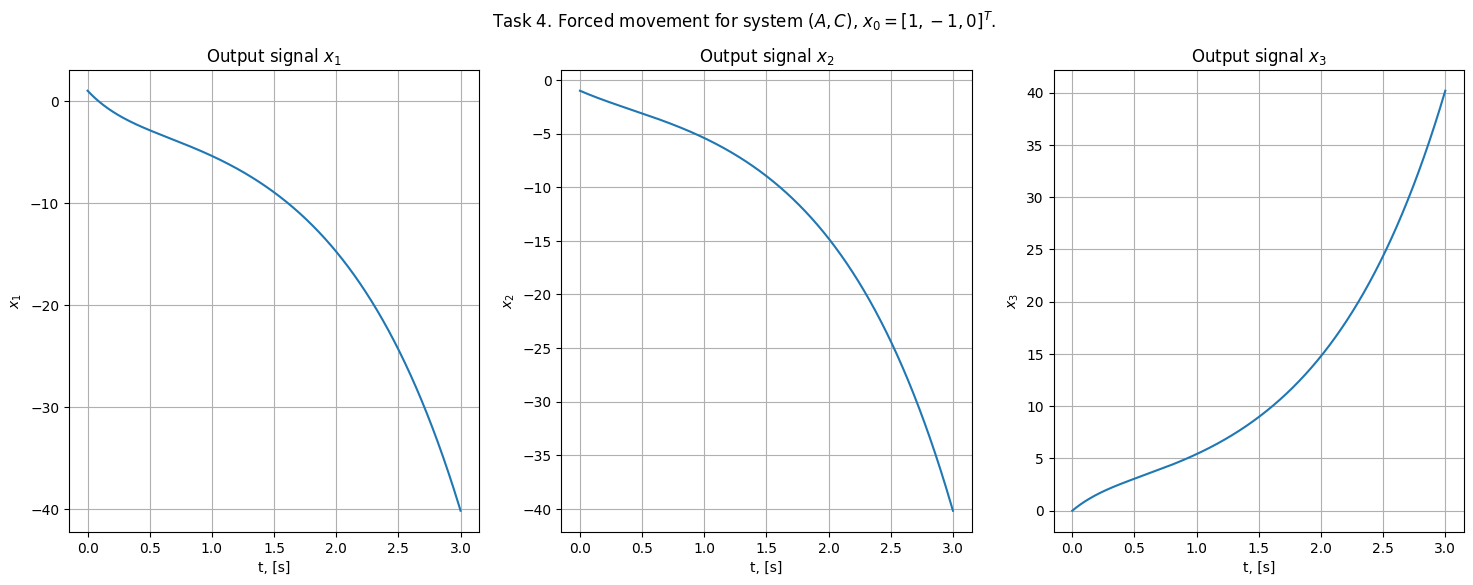
\includegraphics[width=\textwidth]{plot_4_1}
    \caption{\label{fig:The-caption-1}Входной и выходной сигналы системы (задание 4)}
\end{figure}
\pagebreak

\section{Многоканальная система в форме вход-состояние-выход}
Рассмотрим систему вида:
\begin{equation}
    \begin{cases}
        \dot x = Ax + Bu \\
        y = Cx + Du
    \end{cases}
\end{equation}

Согласно заданию, матрицы определяющие систему имеют вид:
\begin{equation*}
    A = \begin{bmatrix}
        0 & -6   \\
        1 &  -4 
        \end{bmatrix}
        B = \begin{bmatrix}
            1 & 9  \\
            3 & 2
            \end{bmatrix}
        C = \begin{bmatrix}
            3 & 5 \\
            2 & 7 
            \end{bmatrix}
        D = \begin{bmatrix}
             0 & 0 \\
             0 & 0
            \end{bmatrix}
\end{equation*}

Выполним моделирование системы:
\begin{lstlisting}[language=Python]
state_space_5 = ctrlmat.ss(A_5, B_5, C_5, D_5)
modeling_time_5 = 20 
time_5 = np.linspace(0,modeling_time_5,int(modeling_time_5/dt))
u_5_1 = np.ones_like(time_5) 
u_5_2 = 2 * np.sin(time_5)
u_5 = np.array([u_5_1, u_5_2])
init_state_5 = [0, 0]
y_5 = ctrl.forced_response(state_space_5, U=u_5, X0=init_state_5, T=time_5).outputs
\end{lstlisting}

\begin{figure}[h]
    \centering
    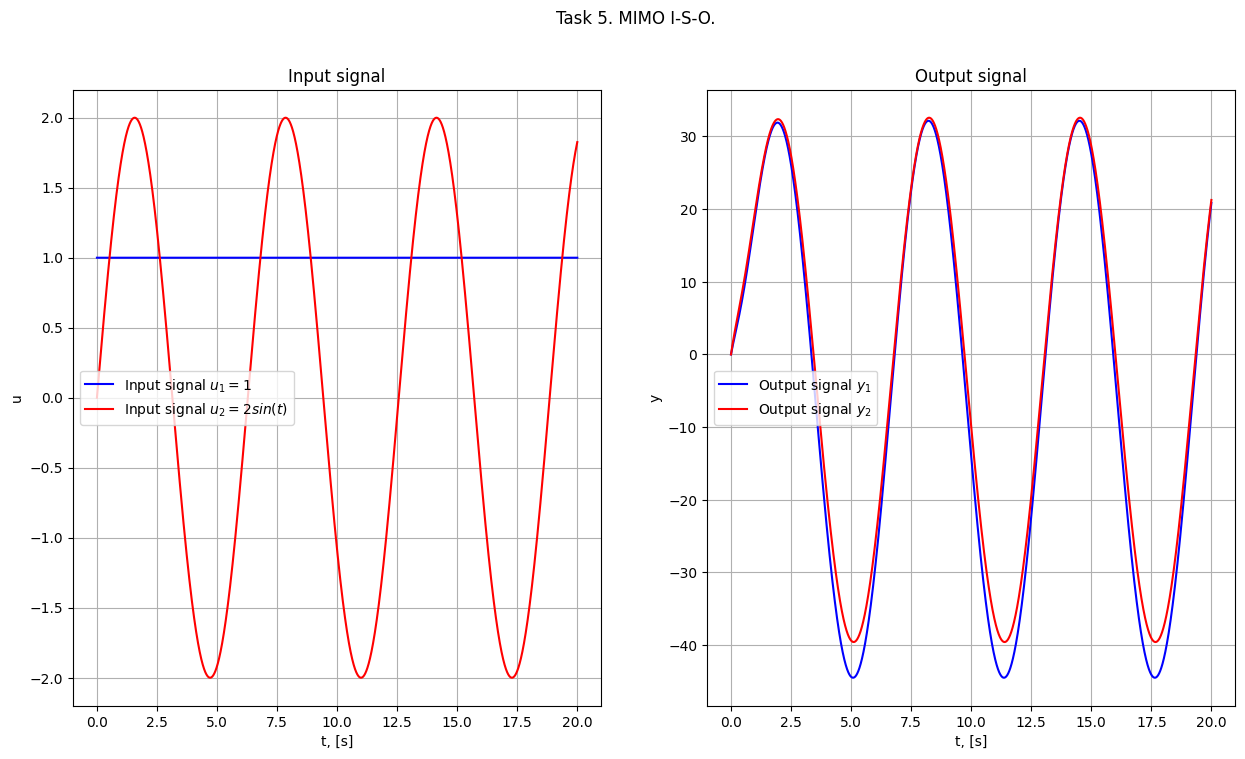
\includegraphics[width=\textwidth]{plot_5_1}
    \caption{\label{fig:The-caption-1}Входные и выходные сигналы системы (задание 5)}
\end{figure}
\pagebreak

\section{Выводы}
\pagebreak